\documentclass[a4paper]{article}
\usepackage{fancyhdr}
\usepackage[backend=bibtex, style=authoryear, uniquename=init, giveninits=true, maxbibnames=3, minbibnames=2]{biblatex} 
\usepackage{lastpage}
\usepackage[utf8]{inputenc}
\usepackage[official]{eurosym}
\usepackage[right=25mm,left=25mm,top=20mm,bottom=20mm]{geometry} 
\usepackage{graphicx} % support the \includegraphics command and options
\usepackage{amsmath}
\usepackage{amssymb}
\usepackage{adjustbox}
\usepackage{mathtools}
\usepackage{subcaption}
\usepackage{centernot}
\usepackage[parfill]{parskip} % Activate to begin paragraphs with an empty line rather than an indent
\usepackage{booktabs} % for much better looking tables
\usepackage{array} % for better arrays (eg matrices) in maths
\usepackage{paralist}% very flexible & customisable lists (eg. enumerate/itemize, etc.)
\usepackage{verbatim} % adds environment for commenting out blocks of text & for better verbatim
\usepackage[table,xcdraw]{xcolor}
\usepackage{perpage}
\usepackage{hyperref}
\usepackage[perpage,symbol*]{footmisc}
\usepackage{chngcntr}
\usepackage{amsthm}
\usepackage{makecell}
\usepackage{csquotes}
\usepackage[nottoc,numbib]{tocbibind}
\counterwithin{figure}{section}
\counterwithin{equation}{section}
\counterwithin{table}{section}
\allowdisplaybreaks
\linespread{1.2}
\pagenumbering{arabic}
\title{Who smokes?}
\author{Samuel Hashem Zehi}
\date{Student ID: 1591277}
\theoremstyle{definition}
\newtheorem{definition}{Definition}[section]
\newtheorem{concept}{Concept}
\newtheorem{lemma}{Lemma}[section]
\newtheorem{rmrk}{Remark}[section]
\newtheorem{note}{Note}[section]
\renewcommand{\thefootnote}{\fnsymbol{footnote}}
\newcommand*\diff{\mathop{}\!\mathrm{d}} %Integral d 
\newcommand{\mbg}{\overset{!}{>}} %must be greater
\newcommand{\mbeq}{\overset{!}{=}} %must be equal
\newcommand{\mnbq}{\overset{!}{\neq}}  %must be unequal
\newcommand{\df}{\partial} %partial derivatives
\newcommand{\fr}{\frac} %fractions
\DeclareMathOperator*{\argmax}{argmax} %argmax proper
\DeclareMathOperator*{\argmin}{argmin} %argmin proper
\newcommand{\uline}{\underline} %underline
\newcommand{\bpm}{\begin{pmatrix}} %matrix shortcuts 4x
\newcommand{\epm}{\end{pmatrix}}
\newcommand{\bbm}{\begin{bmatrix}}
\newcommand{\ebm}{\end{bmatrix}}
\newcommand{\beq}{\begin{equation}} %equation 
\newcommand{\eeq}{\end{equation}}
\newcommand{\beqq}{\begin{equation*}} %unnumbered equation 
\newcommand{\eeqq}{\end{equation*}}
\newcommand{\hbeta}{\hat{\beta}} %estimator for beta
\newcommand{\e}{\epsilon}
\newcommand{\sbdist}{\Sigma_{\sqrt{n}(\hat{\beta}-\beta)}} %Covarianz Matrix for distribution 
\newcommand{\convdist}{\overset{d}{\longrightarrow}} %convergence in distribution
\newcommand{\convprob}{\overset{p}{\longrightarrow}} %convergence in probability
\newcommand{\asymdist}{\overset{a}{\sim}} %asymptotically distributed
\newcommand{\x}{\times} %matrix and vector dimension notation, e.g. x is a k \x 1 vector of regressors
\DeclareCiteCommand{\citeauthorfirstlast}
  {\boolfalse{citetracker}%
   \boolfalse{pagetracker}%
   \DeclareNameAlias{labelname}{first-last}%
   \usebibmacro{prenote}}
  {\ifciteindex
     {\indexnames{labelname}}
     {}%
   \printnames{labelname}}
  {\multicitedelim}
  {\usebibmacro{postnote}}

\DeclareCiteCommand{\citeauthorlastfirst}
  {\boolfalse{citetracker}%
   \boolfalse{pagetracker}%
   \DeclareNameAlias{labelname}{last-first}%
   \usebibmacro{prenote}}
  {\ifciteindex
     {\indexnames{labelname}}
     {}%
   \printnames{labelname}}
  {\multicitedelim}
  {\usebibmacro{postnote}}
\hypersetup{colorlinks, citecolor=black, filecolor=black, linkcolor=black, urlcolor=black} %%for links to not be visible
\bibliography{ideas}
\begin{document}
\begin{titlepage}
\vspace*{0.8cm}
\begin{figure}[!h]
\centering

\includegraphics[width = 0.5\textwidth]{Uni_Logo_2016.png}
\end{figure}
\begin{center}

\vspace*{1,2cm}

\huge {\bfseries Search Interest for Gold Prices and Realized Gold Prices}\\[1.8cm]

\Large {Macroeconometrics}\\[1cm]
\end{center}
\vspace{2cm}

\noindent \textbf{Supervisor:}\\
Univ.-Prof.\ Dipl.-Ing.\ Dr.\ Robert Kunst\\

\vspace{1cm}

\noindent \textbf{Authors:}\\
Hashem Zehi, Samuel (Student ID 12012285) \\
Hochholzer, Matthias (Student ID 11724853) \\

\vspace{1cm}

\noindent Master of Science Economics (M.Sc.)\\

\vspace{1cm}

\noindent Vienna, \today

\setcounter{page}{0}\clearpage
\end{titlepage}
\newpage
\tableofcontents
\newpage
\section{Introduction}
This project investigates the relationship between the realized price of gold and a standardized index measuring the relative online search interest for gold prices. More specifically, can search interest help improve prediction of one-period ahead gold prices. Due to the technological advances in the financial industry nowadays more and more algorithms work based on internet sentiment in order to buy and sell financial products. One possible measure for such automated algorithms is using data provided by companies like Google or Microsoft. Large spikes in search interest may trigger such algorithms. As financial news outlets like Bloomberg or the Financial Times write articles on price changes more and more people will look up prices of goods and commodities, again triggering the algorithms, resulting in a feedback loop. 

This paper is structured as follows. First we explain the data collection process then do some exploratory data analysis. Then we attempt to find the best prediction model for gold prices. Afterwards we model the gold price and the relative search interest jointly. Lastly we give some closing remarks on our results and issues with modeling and data.
\section{Data}
The data used in this project comes from two sources. Firstly the gold price search interest is provided to the public by \citeauthor{Google.2021} (\citeyear{Google.2021}). This data is standardize to a range from zero to 100 over the entire time range. 100 represents the point in time with the highest search interest and zero either no interest at all or simply not enough data for this specific point in time. 50 then simply means that the popularity is at 50\% of the peak value. Due to the ability to collect a wide range of data on the users of the website Google removes datapoints where the same user looked the term up multiple times within a short period of time. Furthermore, regional differences  are accounted for due to the data only being relative search interest, thus regions with larger populations and particular search interests cannot skew the data. It is noteworthy that if the data is split up by regions India, one of the largest markets for gold, appears to have the highest relative search interest, with only countries like Oman, Pakistan, and Myanmar being close. For this analysis we focus on the worldwide interest in the search term \textquote{gold price} over the period 2004 until June 2021.

Secondly, the data on gold prices is provided by \citeauthor{ICEBenchmarkAdministrationLimited.} (\citeyear{ICEBenchmarkAdministrationLimited.}) and published for use by the Economic Research Division of the Federal Reserve Bank St.\ Louis and collected by the London Bullion Market Association. The price is set twice daily, in the morning and the afternoon, and measured in US dollars per troy ounce. For our analysis we use the afternoon price given two separate frequencies. When not modeling the data jointly we use a daily frequency as it allows us to make a more detailed analysis and gives a more accurate reflection of the volatility. It should be noted that there around 200 of the 5,300 observations contain \textquote{NA} values. As there appears to be not specific pattern such as for example no prices being reported on weekends, we have elected to replace these values with the price from the previous day.  

In the joint modeling we are constrained by the frequency with which Google makes search interest data available: monthly. Thus we use a monthly frequency for the realized prices as well, to be more precise we use the prices at the end of each month. 
\newpage
\section{Gold Price Modeling}
In this section look at the daily price of gold. 
%
%
% Add stuff about gold price
%
% Now: first-differenced

Now we consider the first-differenced gold prices.
	\begin{figure}[!t]
	\centering
	\caption{Daily Gold Prices (First-Differences)}
	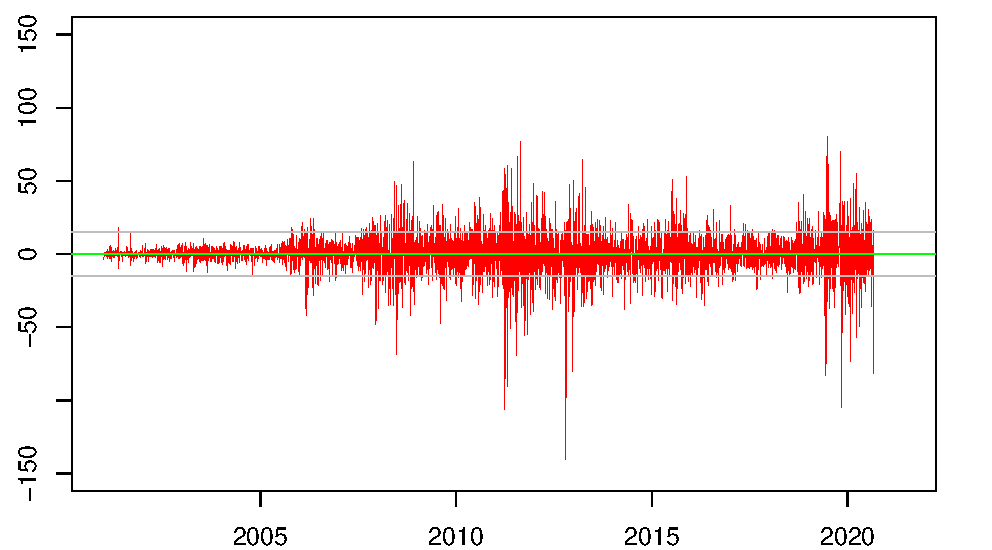
\includegraphics[width=0.90\textwidth]{goldFDHFalone.pdf}
	\end{figure}
At first glance they appear to be stationary around zero with phases of higher and lower volatility. The overall level of volatility appears to have increased starting from 2006 onward, as indicated by the gray lines. Before 2006 there were very few observations outside of the $\pm 15$ band, compared to this occurring very frequently afterwards. In order to illustrate the high frequency of data we chose very thin lines for Figure 3.X. 
% adjust figure name!
It appears that there is some volatility clustering in the daily prices of gold. Four clusters appear very prominent, namely one at around 2007-2008, 2011, 2013, and 2019-2020. Every now and then there are very large outliers, one notable in 2013 with a day-on-day decrease by over USD 100.
% add stuff on unit root test for FDs





\newpage
\subsection{Best-Prediction Modeling}
% add stuff about why PACF/ACF
\begin{figure}[t]
     \centering
     \caption{Empirical (Partial) Autocorrelation Functions of the Gold Price FDs}
     \begin{subfigure}[t]{0.45\textwidth}
         \caption{ACF}        
         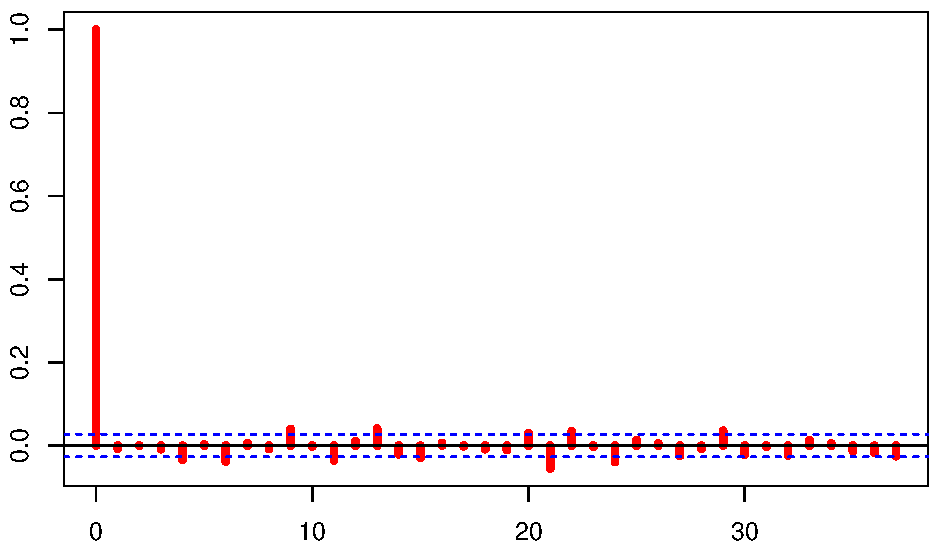
\includegraphics[width=\textwidth]{acfGOLDFD}
    \end{subfigure}
    \begin{subfigure}[t]{0.45\textwidth}
         \caption{PACF}
         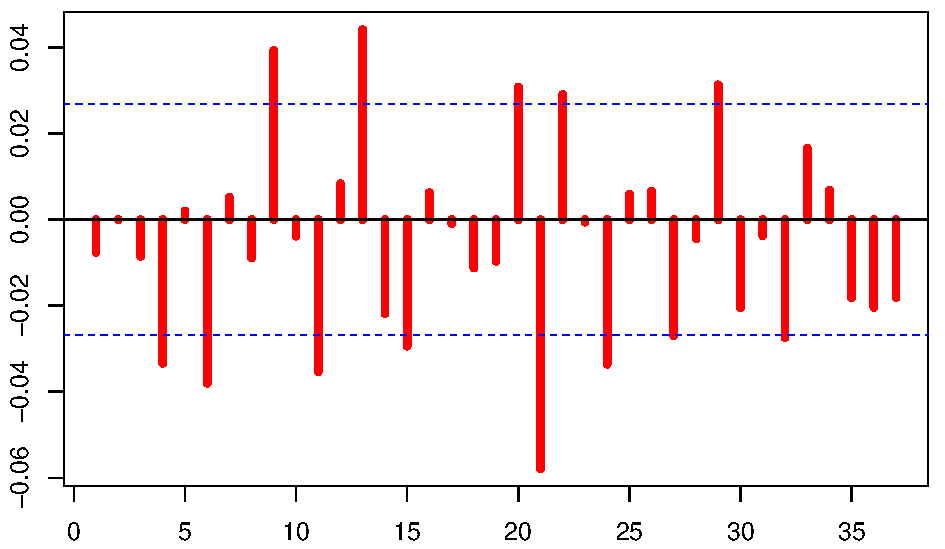
\includegraphics[width=\textwidth]{pacfGOLDFD}
    \end{subfigure}
\end{figure}

In this section we use the AIC in order to determine the optimal lag order. As our data are of somewhat high frequency over a longer period of time, any concerns over the performance of the information criterion in small samples can be disregarded. When modeling prices we are often concerned with trying to predict prices, which justifies the choice of the AIC as it selects the best-forecasting model in large samples rather than leading to a consistent choice of lag orders. We estimate all ARIMA($p,q$) models within a range of $p$ and $q$ values and then choose the one with the lowest AIC value, where the criterion is defined as follows:
	\begin{align*}
	\text{AIC} = \log \hat\sigma^2 + 2 \frac{p+q+1}{2}.
	\end{align*}

\subsection{Volatility Analysis}
As mentioned in the exploratory analysis of the data it does not appear as if the autocovariance is constant over time. Thus it is a natural consequence to further look at ways of modelling the volatility. We do so by considering (G)ARCH models.


	\begin{itemize}
 		\item ARCH: $E({\epsilon_t}^2 | \mathcal{I}_{t-1})= {\sigma_t}^2 = 119.54 + 0.11 {\epsilon_{t-1}}^2$
 		\item GARCH: $E({\epsilon_t}^2 | \mathcal{I}_{t-1})= {\sigma_t}^2 = 0.14 + 0.07 {\epsilon_{t-1}}^2 + 0.93 {\sigma_{t-1}}^2$, according to t-series (slight difference with the "rugarch" package)
  		\item iGARCH: $E({\epsilon_t}^2 | \mathcal{I}_{t-1})= {\sigma_t}^2 = 0.16 + 0.07 {\epsilon_{t-1}}^2 + 0.93 {\sigma_{t-1}}^2$
		\item eGARCH: $log\ {\sigma_t}^2 = 0.02 +0.04\ \frac{| \epsilon_{t-1}|}{\sigma_{t-1}} + 0.10\ log\ {\sigma_{t-1}}^2+ 0.13\ \frac{ \epsilon_{t-1}}{\sigma_{t-1}} $
	\end{itemize}


According to the customary tool AIC, GARCH(1,1), eGARCH(1,1) and iGARCH(1,1) outperform ARCH(1). We would opt for the simplest, the GARCH(1,1) model. The eGARCH model, however, could give quite reasonable results for prizes.

\newpage
\section{Joint Modeling for Gold and Search Interest Index}
\subsection{Exploratory Analysis of the Gold Search Interest Index}
We start by looking a bit closer at the search interest index. This is plotted over the entire observational period available in Figure 4.1.
	\begin{figure}[!t]
	\centering
	\caption{Relative Search Interest in the Term \textquote{gold price} from 2004-2021}
	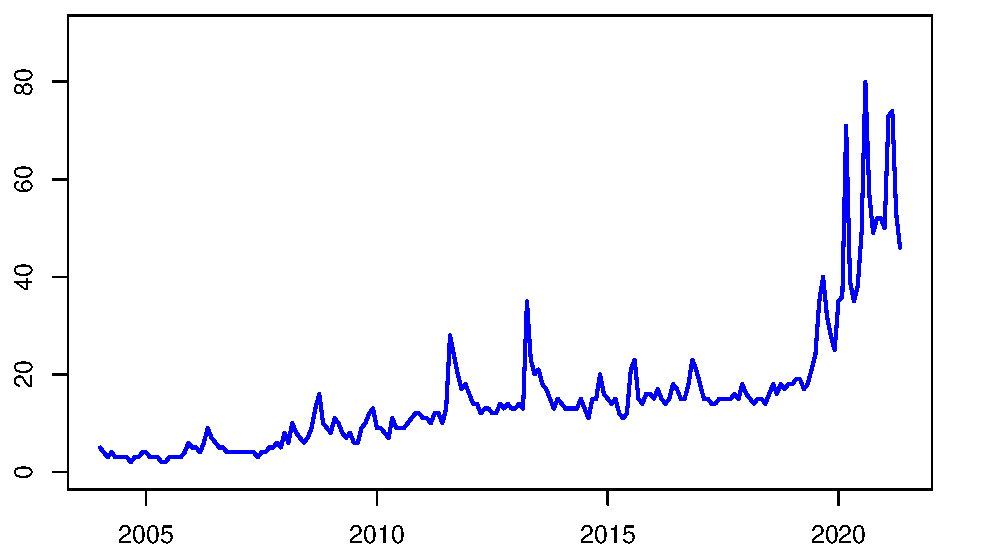
\includegraphics[width=0.90\textwidth]{GoldSearchAlone}
	\end{figure}
It is easy to see that there was a slight upwards trend in the data over the period from 2004 to 2019. In this period there are two spikes in the data, one around late 2012 and one around late 2013 - early 2014. According to \citeauthor{Desk.24062016} (2016) the first spike appears around the time right before the wedding and festival season in India coinciding with a weak local currency. A similar line of reasoning appears to be the reason for the spike in late 2013 - early 2014. Around late 2019 there appears to be a very strong search interest increase, joint with an increase in volatility. This however is not particularly surprising as gold is often hailed as a good, safe investment in times of increased uncertainty. It is likely that political unrest in India, followed by the start of the Corona crisis are the main drivers for this development. Skepticism about the effects of loosened monetary policy on the worth of local currencies in large parts of the world may lead to a flight from local currencies to gold due to its historically stable value. 
%

\subsection{VAR Model for Gold Price and Search Interest Index}
%
\newpage
\section{Conclusion}
%
%
%
%
%
%
%
%
\newpage
\addcontentsline{toc}{section}{References}
\section*{References}
\printbibliography
% add google and FRED
\end{document}